\begin{table}
  \caption{Parameters of the die and package.}
  \label{tab:parameters}
  \centering
  \begin{tabular}{|l|r|}
    \hline
    Parameter & Value \\
    \hline
    \hline
    Ambient temperature                   &   27 ${}^\circ C$ \\
    Convection capacitance                & 140.4 J/K \\
    Convection resistance                 & 0.1 K/W \\
    Die thickness                         & 0.15 $mm$ \\
    Thermal interface material thickness  & 0.02 $mm$ \\
    Heat spreader side                    &   20 $mm$ \\
    Heat spreader thickness               &    1 $mm$ \\
    Heat sink side                        &   30 $mm$ \\
    Heat sink thickness                   &   15 $mm$ \\
    \hline
  \end{tabular}
  \vspace{15pt}
\end{table}
The equivalent circuit of a multiprocessor system with a thermal package can be built in different ways depending on the intended level of details. Consequently, the number of nodes $N_n$ and structure of the matrices $\m{C}$ and $\v{G}$ in \equref{eq:fourier-model} depend on the particular model. Thermal nodes that belong to the package are called inactive in the sense that their power dissipation is assumed to be zero.

Without loss of generality, in this paper we use thermal circuits where each of the $N_p$ processing elements is captured by one thermal node \cite{huang2003}. In the model, three cooling layers are present, namely the thermal interface material, heat spreader, and heat sink captured by $N_p$, $N_p + 4$, and $N_p + 8$ inactive thermal nodes, respectively. Therefore, the total number of thermal nodes $N_n$ is $4 \times N_p + 12$. The parameters of the die and thermal package, used through out this paper, are given in \tabref{tab:parameters}.

A simplified example of such a thermal circuit for a dual-core architecture is depicted in \figref{fig:circuit}. It can be seen that the inter-core thermal influence is taken into account by modeling the heat flux between the cores (the top two thermal nodes) with the corresponding thermal resistance.

Some or all cores can be also modeled at a finer level of granularity, where caches, ALUs, or registers will be captured as individual thermal nodes.
\begin{figure}
  \vspace{10pt}
  \centering
  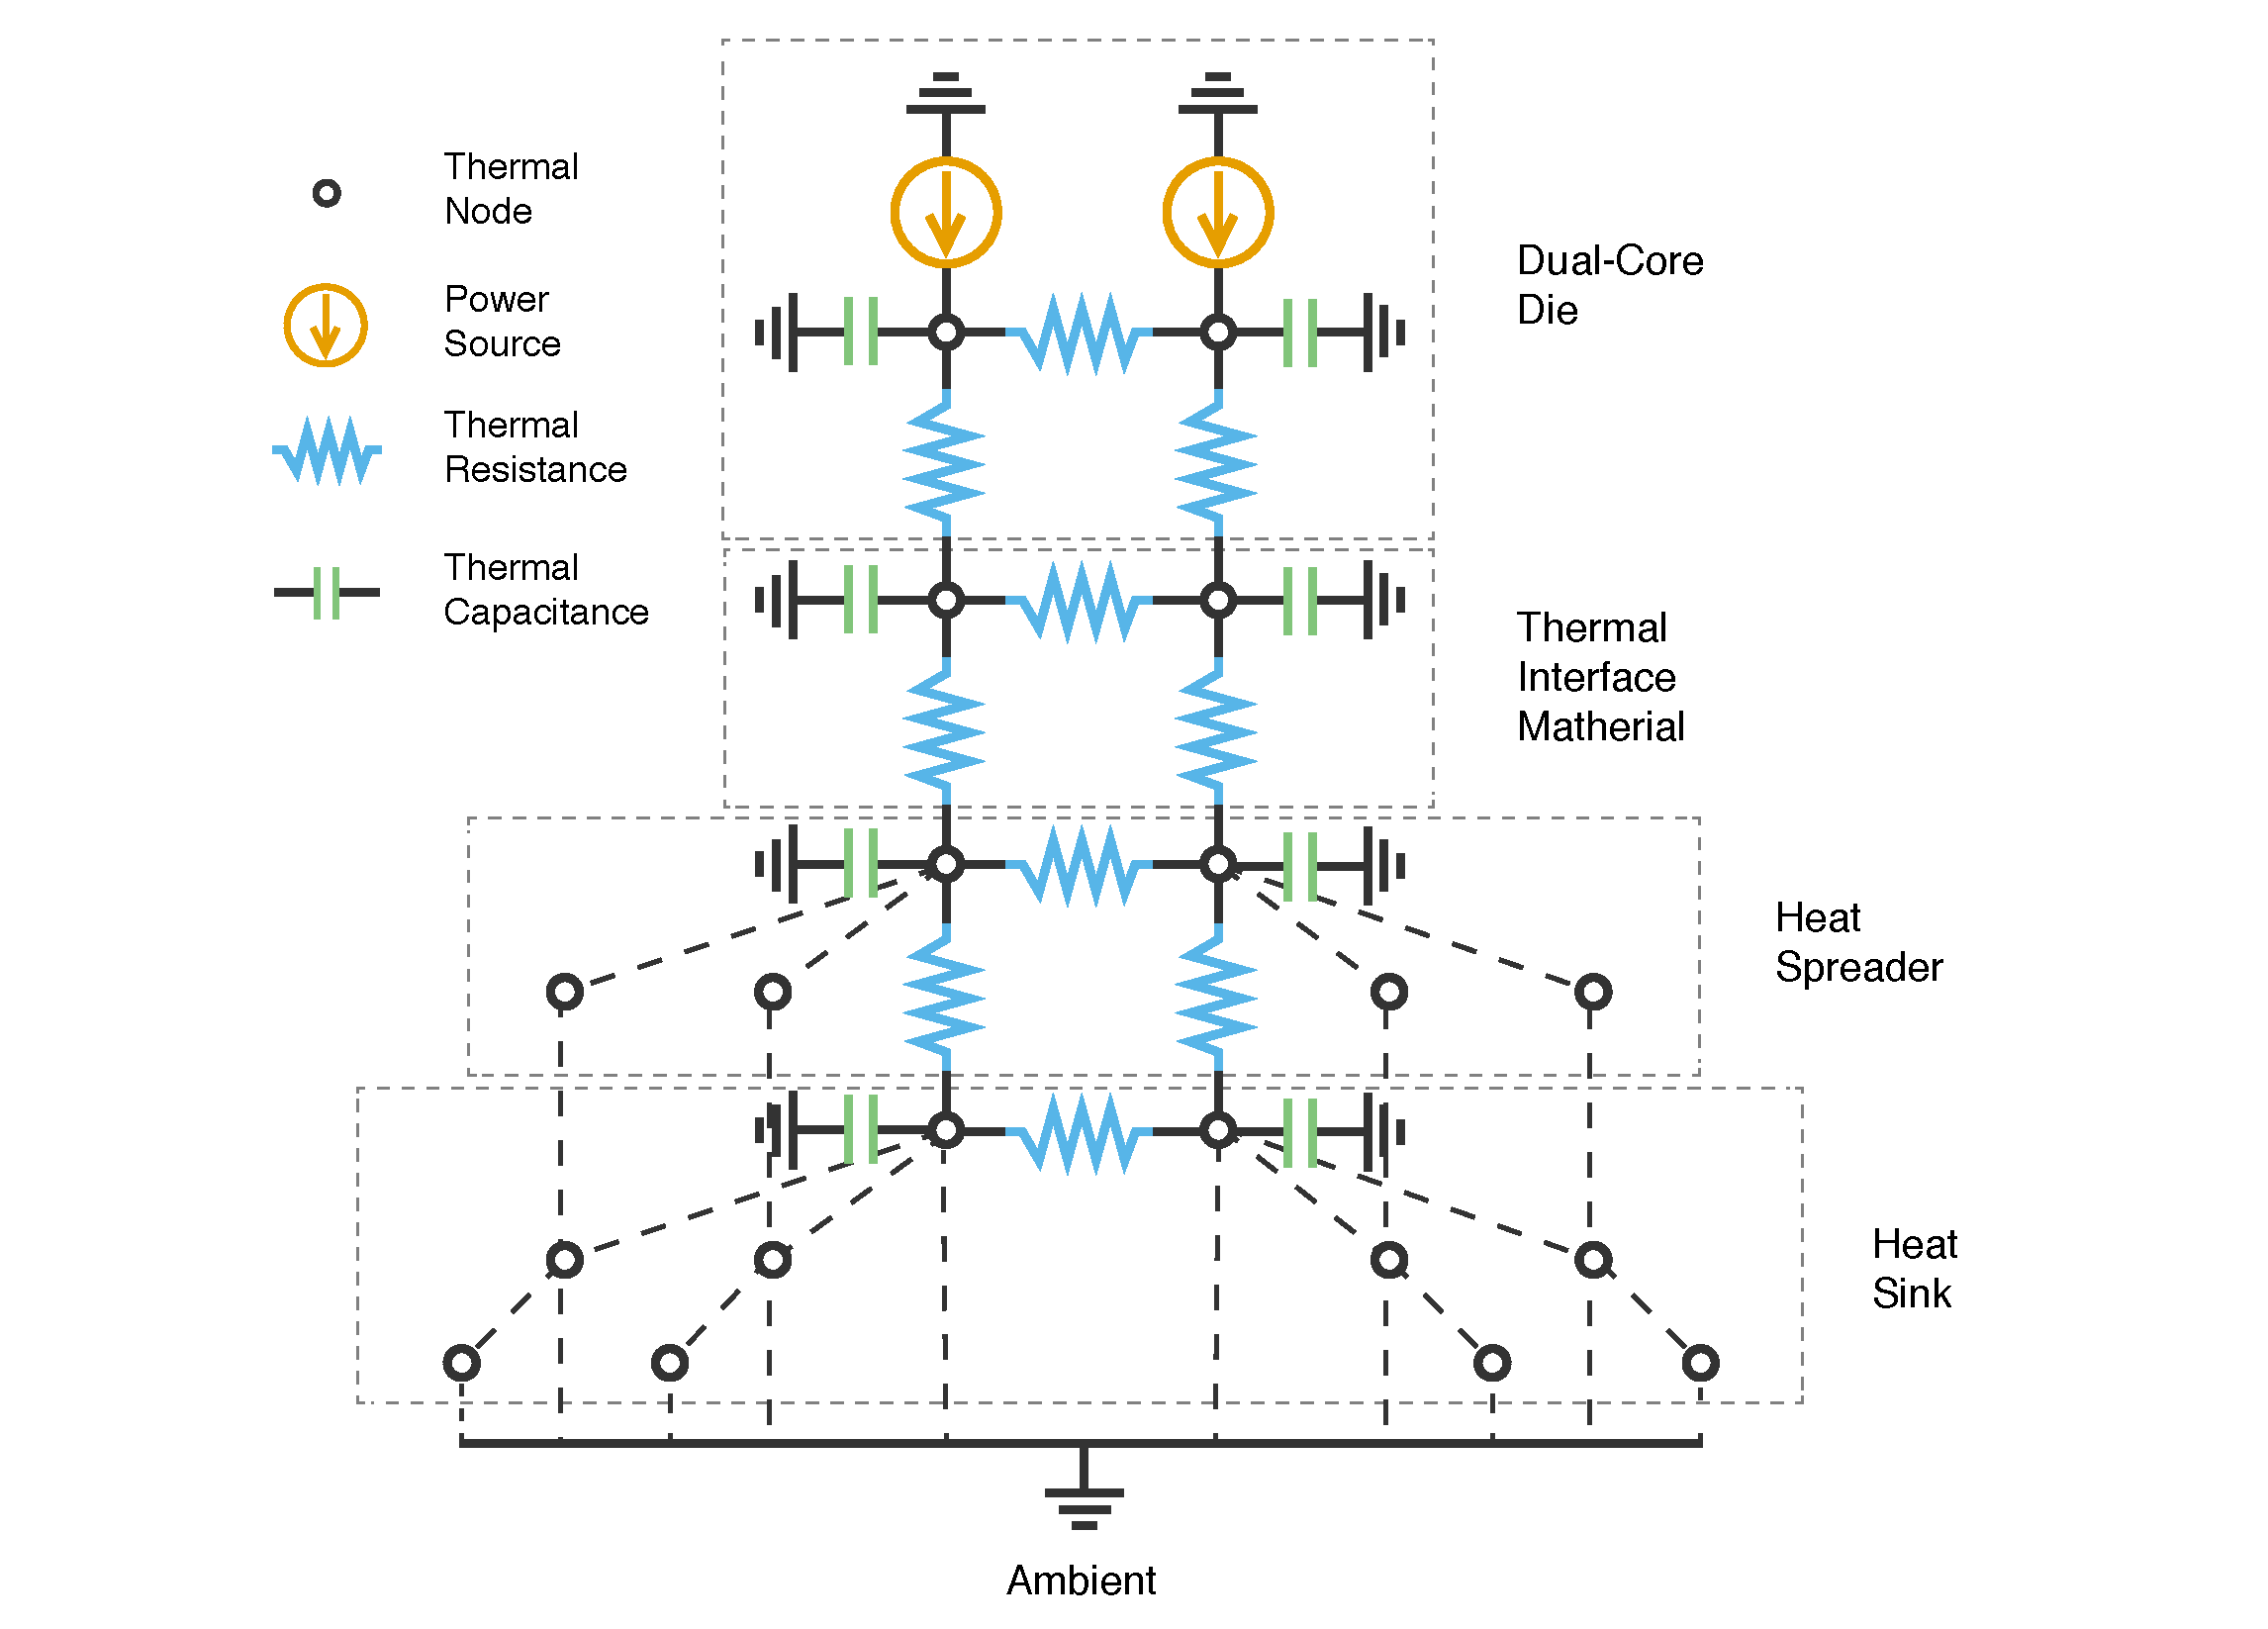
\includegraphics[width=\linewidth]{assets/circuit.pdf}
  \caption{Equivalent RC thermal circuit.}
  \label{fig:circuit}
  \vspace{15pt}
\end{figure}
